\documentclass{exam}

\usepackage{units} 
\usepackage{graphicx}
\usepackage[fleqn]{amsmath}
\usepackage{cancel}
\usepackage{float}
\usepackage{mdwlist}
\usepackage{booktabs}
\usepackage{cancel}
\usepackage{polynom}
\usepackage{caption}
\usepackage{fullpage}
\usepackage{xfrac}
\usepackage{enumerate}

\newcommand{\degree}{\ensuremath{^\circ}} 
\everymath{\displaystyle}

\printanswers

% \begin{figure}[H]
%   \centering
%   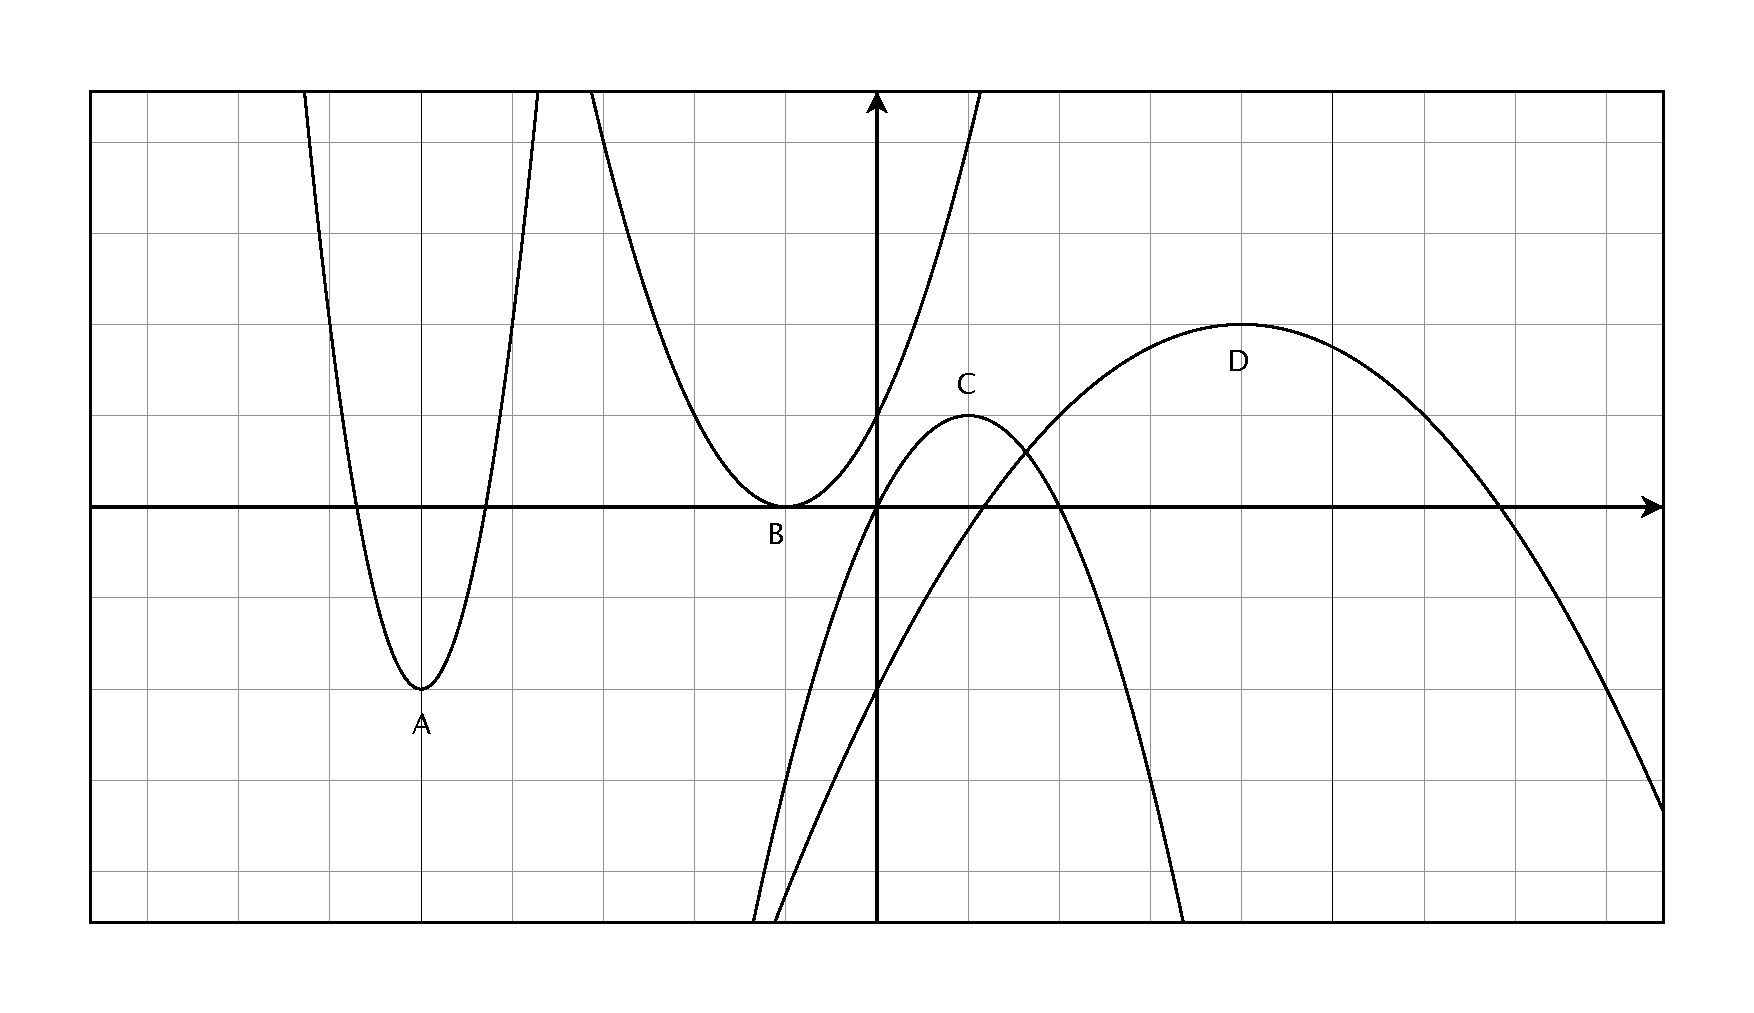
\includegraphics[scale=.3]{problem_7.eps}
%   \caption*{Problem 7}
% \end{figure}

% \begin{tabular}{cc}
% \toprule
% period & amplitude \\
% \midrule
%   $\pi$ & $2$ \\
% \bottomrule
% \end{tabular}

\title{Math 141 Notes \\ Section 4.4}

\date{June 26, 2013}

\begin{document}

  \maketitle
  \tableofcontents

  \section{Equations with Exponentials}

  \subsection{One Exponential Term}
  example:
  \begin{align*}
    2^x - 8 &= 0 \\
    2^x     &= 8 \\
    x       &= \log_2 8 \\
            &= 3 \\
  \end{align*}

  \begin{itemize}
    \item isolate power on one side
    \item take logarithm of both sides 
  \end{itemize}

  \begin{align*}
    2^{2x} - 16 &= 0 \\
    2^{2x}      &= 16 \\
    2x          &= \log_2 16 \\
                &= 4 \\
    x           &= 2 \\
  \end{align*}

  alternate:
  \begin{align*}
    2^{2x} - 16 &= 0 \\
    2^{2x} &= 16 \\
    4^x &= 16 \\
    x       &= \log_4 16 \\
            &= 2 \\
  \end{align*}

  \subsection{Exponential/Powers Combined}
  \begin{align*}
    2^x x^2 - 2^x &= 0 \\
    2^x \left( x^2 - 1 \right) &= 0 \\
    2^x (x + 1)(x - 1) &= 0 \\
    x &= \{ -1, 1 \}
  \end{align*}

  procedure:
  \begin{itemize*}
    \item factor out exponential
    \item solve polynomial as usual
  \end{itemize*}

  \subsection{Exponential With Multiple Terms}
  factor:
  \begin{align*}
    e^{2x} - 6e^x + 8  &= 0 \\
    (e^x - 2)(e^x - 4) &= 0 \\
    x                  &= \{ \ln 2, \ln 4 \} \\
  \end{align*}

  some factors may not produce solutions:
  \begin{align*}
    e^{2x} + 2e^x - 3  &= 0 \\
    (e^x - 1)(e^x + 3) &= 0 \\
    x                  &= 0 \\
  \end{align*}

  procedure:
  \begin{itemize*}
    \item factor 
    \item set each term equal to zero and solve
    \item some terms may have no solution
  \end{itemize*}

  more examples:
  \begin{align*}
    2e^{2x} - e^x - 15  &= 0 \\
    (2e^x + 5)(e^x - 3) &= 0 \\
    x                   &= \ln 3 \\
  \end{align*}

  \begin{align*}
    e^{4x} - 16                    &= 0 \\
    (e^{2x} - 4)(e^{2x} + 4)       &= 0 \\
    (e^x - 2)(e^x + 2)(e^{2x} + 4) &= 0 \\
    x                              &= \ln 2 \\
  \end{align*}

  alternate:
  \begin{align*}
    e^{4x} - 16 &= 0 \\
    e^{4x}      &= 16 \\
    4x          &= \ln 16 \\
    x           &= \frac{\ln 16}{4} \\
                &= \frac{\ln 2}{4} \\
                &= \frac{4 \ln 2^4}{4} \\
                &= \ln 2 \\
  \end{align*}

  \section{Logarithm Equations}

  \subsection{One Term}

  example:
  \begin{align*}
    \log_3 x - 2 &= 0 \\
    \log_3 x     &= 2 \\
    x            &= 3^2 \\
                 &= 9 \\
  \end{align*}

  procedure:
  \begin{itemize*}
    \item isolate logarithm on one side of the equation
    \item write as an exponential (or raise the base to each side)
  \end{itemize*}
  
  another example:
  \begin{align*}
    \log_4 (x - 2) &= 3 \\
    x - 2        &= 4^3 \\
    x            &= 66 \\
  \end{align*}

  \subsection{Multiple Terms}

  \begin{align*}
    2 \log x       &= \log 9 + \log(x - 2) \\
    \log x^2       &= \log [9(x - 2)] \\
    x^2            &= 9x - 18 \\
    x^2 - 9x + 18  &= 0 \\
    (x - 3)(x - 6) &= 0 \\
    x              &= \{ 3, 6 \} \\
  \end{align*}

  procedure:
  \begin{itemize*}
    \item use the rules of logarithms to get one logarithm on each side
    \item drop the logarithms
    \item solve for $x$
    \item verify that all the solutions are in the original domain
  \end{itemize*}

  more examples:
  \begin{align*}
    2 \log x       &= \log 4 + \log(x + 3) \\
    \log x^2       &= \log [4(x + 3)] \\
    x^2            &= 4x + 12 \\
    x^2 - 4x - 12  &= 0 \\
    (x + 2)(x - 6) &= 0 \\
    x              &= 6 \\
  \end{align*}

  \begin{align*}
    \ln x + \ln(x + 1) &= \ln (3x) \\
    \ln [x(x + 1)]     &= \ln (3x) \\
    x^2 + x            &= 3x \\
    x^2 - 2x           &= 0 \\
    x(x - 2)           &= 0 \\
    x                  &= 2 \\
  \end{align*}

  \begin{align*}
    \ln x          &= \ln 21 - \ln(x - 4) \\
    \ln x          &= \ln \frac{21}{x - 4} \\
    x              &= \frac{21}{x - 4} \\
    x^2 - 4x       &= 21 \\
    x^2 - 4x - 21  &= 0 \\
    (x + 3)(x - 7) &= 0 \\
    x              &= 7 \\
  \end{align*}

  \section{Applications}

  \begin{enumerate}
    \item If you deposit \$10,000 in an account that pays 5\% per year
      
      \begin{enumerate}[a]
        \item when will you have \$15,000?
          \begin{align*}
            15000 &= 10000 e^{.06t} \\
            t     &= \unit[8.1]{year} \\
          \end{align*}

        \item how long will it take for your money to double?
          \begin{align*}
            A     &= P e^{rt} \\
            2P    &= P e^{rt} \\
            2     &= e^{rt} \\
            \ln 2 &= rt \\
            t     &= \frac{\ln 2}{r} \\
            \\
            t     &= \frac{\ln 2}{0.05} \\
                  &= \unit[13.9]{year} \\
          \end{align*}

      \end{enumerate}

    \item {\em Annual Percentage Yield} is simple interest rate for one year equivalent to a compound rate.
      \begin{enumerate}[a]
        \item find APY of 4\% compounded monthly
          \begin{align*}
            A &= P \left( 1 + \frac{.04}{12} \right)^{12} \\
              &= 1.04074 P \\
          \end{align*}

          The APY is 4.074\%

        \item find APY of 4\% compounded continuously
          \begin{align*}
            A &= P e^r \\
              &= 1.0408 P \\
          \end{align*}

          The APY is 4.081\%

      \end{enumerate}

    \item
      How long would it take \$10,000 to grow to \$15,000 if the interest is 5\% compounded quarterly?
      \begin{align*}
        15,000  &= 10,000 \left( 1 + \frac{0.05}{4} \right)^{4t} \\
        1.5     &= (1.0125)^{4t} \\
        \ln 1.5 &= 4t \ln 1.0125 \\
        t       &= \frac{\ln 1.5}{4 \ln 1.0125} \\
        t       &= \unit[8.16]{year} \\
      \end{align*}

    \item
      If \$10,000 was invested for 5 years with interest compounded semi-annually.  At the end of 5 years, the sum
      was \$15,000.  What was the interest rate?

      \begin{align*}
        15,000 &= 10,000 \left( 1 + \frac{r}{2} \right)^{10} \\
        r      &= 0.0828 \\
      \end{align*}

    \item
      What was the interest rate if the interest was compounded continuously?

      \begin{align*}
        15,000 &= 10,000 e^{5r} \\
        r      &= 0.0811
      \end{align*}

    \item
      Carbon 14 has a half-life of 8,000 years.  If 40\% of the original carbon remains, how old is the sample?

      \begin{align*}
        \frac{0.5} &= e^{-r \cdot 8000} \\
        \ln 0.5    &= -8,000 r \\
        r          &= -0.0000866434 \\
        \\
        0.4 &= e^{-0.0000866434t} \\
        t   &= \frac{\ln 0.4}{-0.0000866434t} \\
            &= \unit[10,575]{year} \\
      \end{align*}


  \end{enumerate}
\end{document}
